\documentclass{article}
\usepackage{subcaption}
\usepackage{graphicx}
\usepackage{mathtools}
\usepackage{amssymb}
\usepackage{setspace}

% code to adjust margins
\addtolength{\oddsidemargin}{-.875in}
	\addtolength{\evensidemargin}{-.875in}
	\addtolength{\textwidth}{1.75in}

	\addtolength{\topmargin}{-.875in}
	\addtolength{\textheight}{1.75in}

\makeatletter

\title{Probability Project Observations}
\author{Omema Ahmed oa04320 \\ Aiman Junaid aj05161 \\ Fatima Zehra fz04316}
\date{\today}
\begin{document}
    \maketitle
    \section*{Task 1}
    To find the expected distance from the starting point (i.e. origin by default or the given coordinates), we ran simulations for 1000 walks and calculated their average.
    Our function increments the distance of a random walk at each step, which is 1 in our case, and returns its sum. Negative coordinates denote movement on left of origin, 
    and positive denote movement on right. To move left, we subtract 1 from x, and to move right we add 1.
    The shape of our resulting graph was a Gaussian curve, which is because binomial converges to Normal distribution. % insert reference to figure
    We tested our model for a range of probabilities, and each gives a different expected distance based on their probabilities and starting position.

    \section*{Task 2}
    To calculate the expected time for two random walks to meet, we calculated the total steps it took both of them to reach the same x-coordinate, and ran simulation for 1000 walks to take average.
    In our function, we started one walk from x=0, and randomly assigned the starting position of second walk. We tested our model for unequal probabilities, for one position being fixed (not moving), 
    and for different starting position of both walks.
    The resulting graph displays that the time it took for most of them to meet, was within 5000 steps.
    
    \section*{Task 3}
    To simulate a 2D random walk, we used matplotlib's animation.We assumed that after reaching 
    the boundary of the circle, if the next position of the walk is beyond the boundary,
    it will reflect back with the distance between the boundary and the new point.
    
    \section*{Task 4}
    We used a uniform random variable, and calculated the step size that ranged between 0-1, using numpy's random.uniform() function.
    Our resulting graph was a Gaussian curve, but in comparison with \textbf{Task 1}, it is smoother as we used continuous values for step.
    Again, we calculated the expected distance using the same method as explained earlier for \textbf{Task 1}.

    \section*{Task 5}
    \section*{Task 6}
    \section*{Task 7}
    \section*{Task 8}
    \section*{Graphs} 
    % How to insert images
    \begin{figure}
        \centering
            \begin{subfigure}[b]{0.5\textwidth}            
                    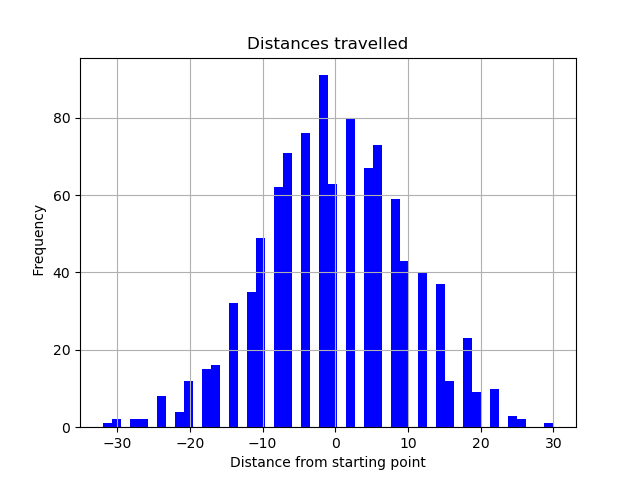
\includegraphics[width=\textwidth]{Graphs/task1.png}
                    \caption{Task 1}
                    % \label{fig:SRl}
            \end{subfigure}%
             %add desired spacing between images, e. g. ~, \quad, \qquad etc.
              %(or a blank line to force the subfigure onto a new line)
            \begin{subfigure}[b]{0.5\textwidth}
                    \centering
                    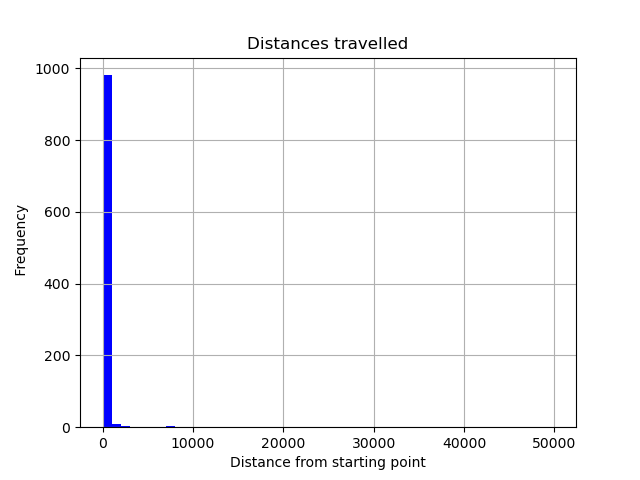
\includegraphics[width=\textwidth]{Graphs/task2.png}
                    \caption{Task 2}
                    % \label{fig:D-Imager}
            \end{subfigure}
            % \begin{subfigure}[b]{0.5\textwidth}
            %     \centering
            %     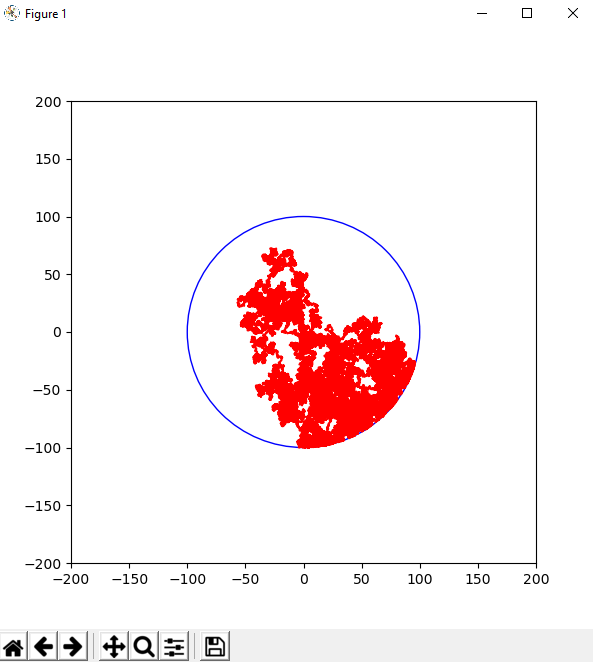
\includegraphics[width=\textwidth]{Graphs/task3.png}
            %     \caption{Task 3}
            %     % \label{fig:D-Imager}
            % \end{subfigure}
            \begin{subfigure}[b]{0.5\textwidth}
                \centering
                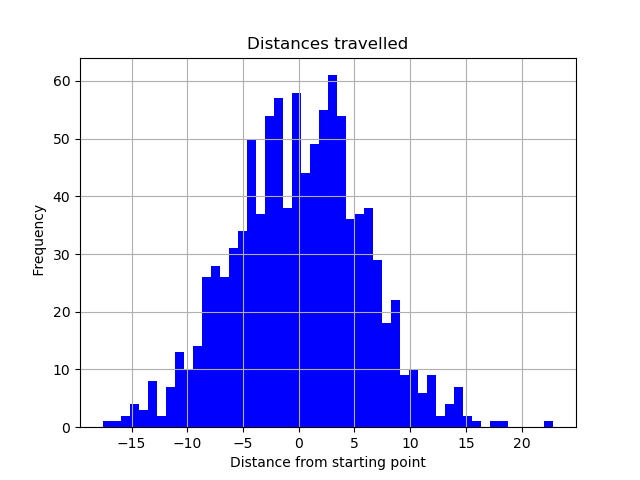
\includegraphics[width=\textwidth]{Graphs/task4.png}
                \caption{Task 4}
                % \label{fig:D-Imager}
            \end{subfigure}
            % \begin{subfigure}[b]{0.5\textwidth}
            %     \centering
            %     \includegraphics[width=\textwidth]{Graphs/task5.png}
            %     \caption{Task 5}
            %     % \label{fig:D-Imager}
            % \end{subfigure}
            % \begin{subfigure}[b]{0.5\textwidth}
            %     \centering
            %     \includegraphics[width=\textwidth]{Graphs/task5.png}
            %     \caption{Task 5}
            %     % \label{fig:D-Imager}
            % \end{subfigure}
            % \begin{subfigure}[b]{0.5\textwidth}
            %     \centering
            %     \includegraphics[width=\textwidth]{Graphs/task7.png}
            %     \caption{Task 7}
            %     % \label{fig:D-Imager}
            % \end{subfigure}
            % \begin{subfigure}[b]{0.5\textwidth}
            %     \centering
            %     \includegraphics[width=\textwidth]{Graphs/task8.png}
            %     \caption{Task 8}
            %     % \label{fig:D-Imager}
            % \end{subfigure}
            % \caption{Graphs}\label{fig:TOF}
    \end{figure}

    
    % How to cite graphs

    % As you can see in the figure \ref{fig:mesh1}, the 
    % function grows near 0. Also, in the page \pageref{fig:mesh1} 
    % is the same example.
    
    \section*{Bibliography}
    % Don't know how to make, refer to probability assignments
\end{document}